% \section{Integrando las nuevas variables al dataset VarQ Curado}

En esta sección buscamos cuantificar en qué medida el esfuerzo realizado a lo largo de esta tesis mejora e impacta sobre nuestro set de datos original (VarQ). Para ello, integraremos al set VarQ Curado, que dispone de 9 features estructurales y 7,418 variantes, los features fisico-químicos y genómicos obtenidos a lo largo de esta tesis.

\section{Creación del dataset Integral+VarQ Curado}
Para generar este dataset cruzamos las variantes de ambos datasets quedándonos con las variantes de VarQ. El dataset resultante posee 73 variables, que corresponden a las 63 variables del dataset Integral sumado a las 9 variables del dataset VarQ Curado y la variable de respuesta. Este dataset posee 7,418 variantes de las cuales 5,377 (72\%) son patogénicas y 2,041 (28\%) son benignas. 

\begin{figure}[H]
    \centering
    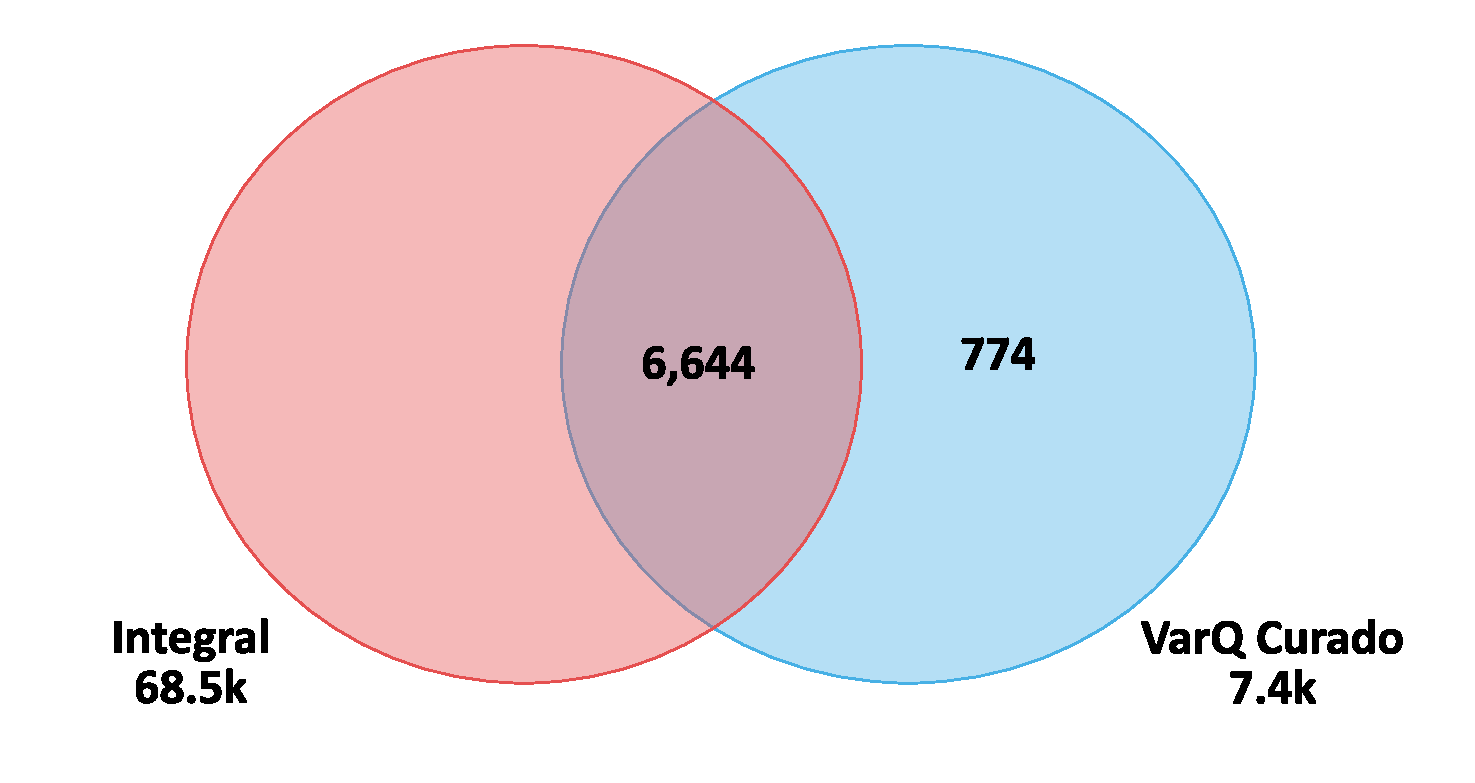
\includegraphics[scale=0.4]{documents/latex/figures/3/integral_varq/interseccion_varq_integral.pdf}
    \caption{.}
    \label{fig:interseccion_varq_integral}
\end{figure}



\section{Generación del Modelo}
Como a lo largo de todo este trabajo, volvimos a repetir el pipeline de Random Forest con imputación de variables continuas con la mediana y con el valor más frecuente en el caso de las variables categóricas. También evaluamos el dataset usando XGBoost de la misma forma que con el modelo Integral. El dataset de entrenamiento posee 4,970 variantes (66\%), y el tercio restante se destinó al dataset de test. Estas variables fueron elegidas al azar, con una semilla pseudoaleatoria para poder replicar el experimento.  

\section{Resultados}
El dataset de test arrojó un AUC de 0.86 para Random Forest y 0.88 con XGBoost, que representa una mejora sensible con respecto al modelo realizado con el dataset VarQ Curado (0.74), sin superar lo obtenido por el dataset Integral (0.90 con XGBoost). Con respecto a las métricas de análisis, en la tabla \ref{tab:metrics_integral_varq} observamos una mejora generalizada, especialmente en la precisión en la detección de variantes benignas, que pasa de 0.57 a 0.81 en el nuevo modelo, y también en el \textit{recall}, que pasa de 0.26 a 0.53. Si bien sigue siendo un número bajo, es posible modificar el \textit{threshold} en la función de decisión para obtener un \textit{recall} más alto sacrificando precisión. 


\begin{table}[H]
\centering
\begin{tabular}{|l|l|l|l|l|l|l|}
\hline
Modelo & Precisión & Recall & AUC & F1-score & $t_{fit}$ & $t_{pred}$ \\ \hline
RF  & 0.84 & 0.95 & 0.87 & 0.89 & 15.4 s & 0.07 s \\ \hline
XGB & 0.86 & 0.94 & 0.88 & 0.90 & 1m 20 s & 0.1 s \\ \hline
\end{tabular}
\label{tab:metrics_model}

\caption{Comparación de métricas de modelos usando el dataset Integral+VarQ Curado. Las variables $t_{fit}$ y $t_{pred}$ corresponden al tiempo de entrenamiento y de predicción de todas las variantes \todo{REFERENCIAR}.}
\end{table}


\begin{table}[H]
\centering
\begin{tabular}{|l|l|l|l|}
\hline
             & Precision & Recall & F1-score \\ \hline
Benignas     & 0.81      & 0.53   & 0.64     \\ \hline
Patogénicas  & 0.84      & 0.95   & 0.89     \\ \hline
Promedio     & 0.83      & 0.83   & 0.82     \\ \hline
\end{tabular}
\caption{Reporte de métricas del modelo Random Forest usando el dataset Integral+VarQ Curado.}
\label{tab:metrics_integral_varq_rf}
\end{table}


\begin{table}[H]
\centering
\begin{tabular}{|l|l|l|l|}
\hline
             & Precision & Recall & F1-score \\ \hline
Benignas     & 0.80      & 0.59   & 0.68     \\ \hline
Patogénicas  & 0.86      & 0.94   & 0.90     \\ \hline
Promedio     & 0.84      & 0.85   & 0.84     \\ \hline
\end{tabular}
\caption{Reporte de métricas del modelo XGB usando el dataset Integral+VarQ Curado.}
\label{tab:metrics_integral_varq_xgb}
\end{table}



\section{Importancia de las variables}
La información proporcionada por la librería acerca de la importancia de las variables en el modelo \textit{scikit-learn} están presentadas en la figura \ref{fig:importances_integral_varq}. En este ranking de las 10 variables más relevantes encontramos otra vez en primer lugar con amplia ventaja a las variables de conservación genómica, aunque también se mantiene la variación de energía y al porcentaje de SASA, que son variables pertenecientes al dataset VarQ Curado y que habían aparecido en el ranking de dicho modelo. 

\begin{figure}[H]
    \centering
    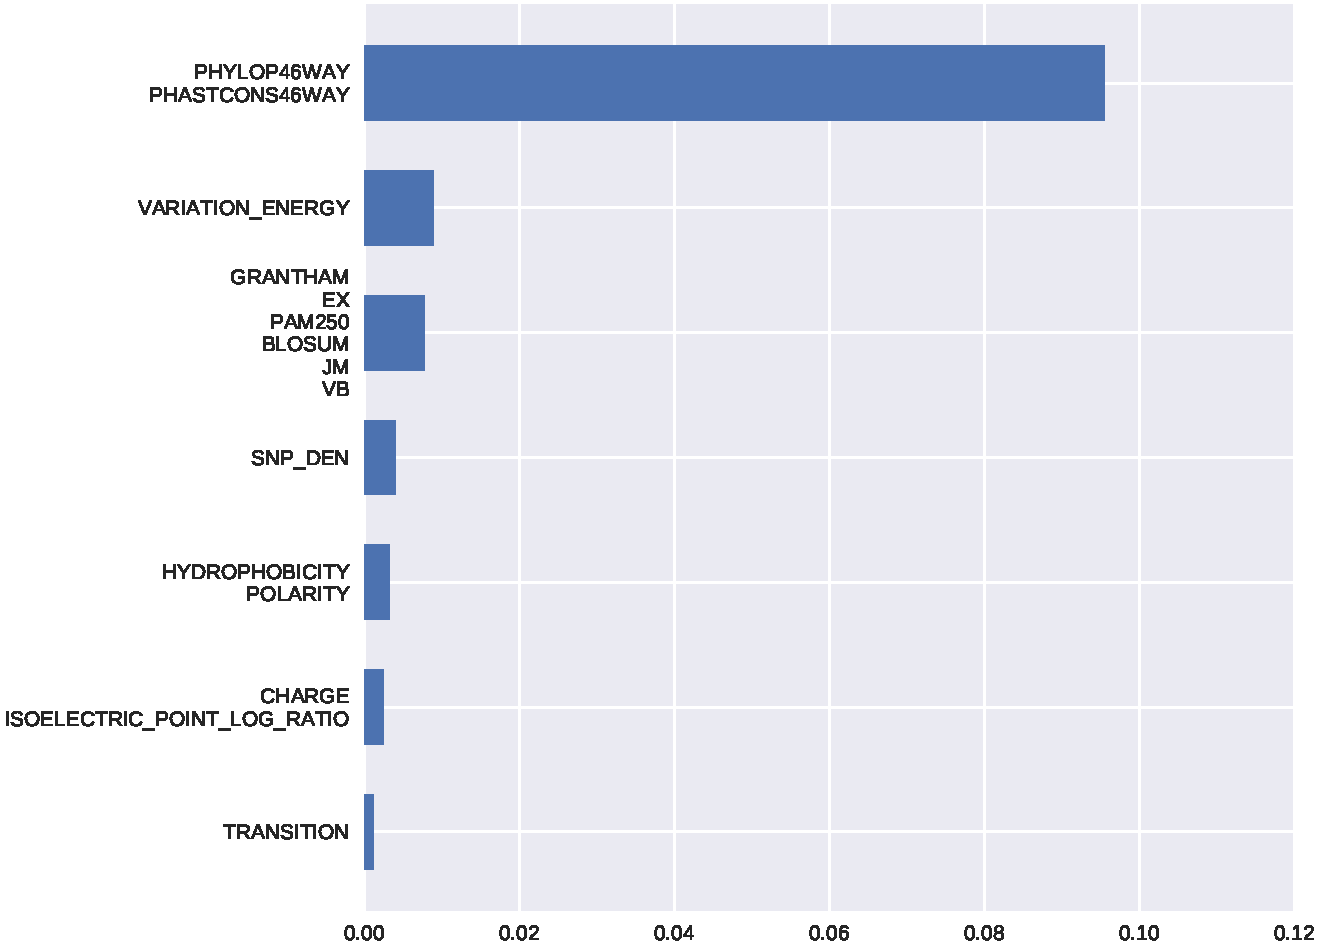
\includegraphics[scale=0.6]{documents/latex/figures/3/integral_varq/integral_varq_importance_cluster.pdf}
    \caption{Variación en la precisión al permutar clusters de variables correlacionadas ($>$ 0.90) del dataset Integral+VarQ Curado usando Random Forest.}
    \label{fig:importance_cluster_integral_varq}
\end{figure}

\begin{figure}[H]
    \centering
    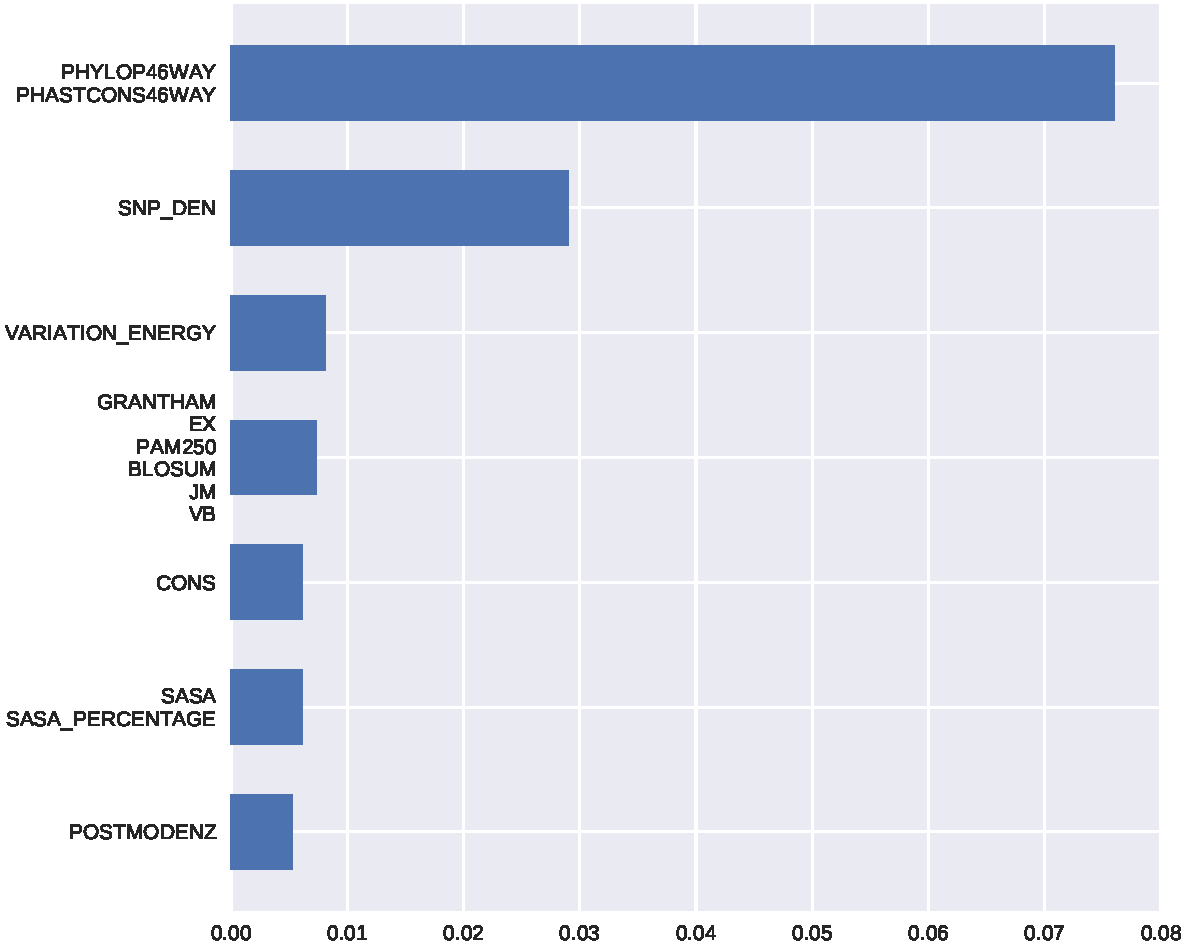
\includegraphics[scale=0.6]{documents/latex/figures/3/integral_varq/integral_varq_importance_cluster_xgb.pdf}
    \caption{Variación en la precisión al permutar clusters de variables correlacionadas ($>$ 0.90) del dataset Integral+VarQ Curado usando XGB.}
    \label{fig:importance_cluster_integral_varq_xgb}
\end{figure}


\newpage
\begin{figure}[H]
\centering
\begin{subfigure}[b]{0.7\textwidth}
    \centering
    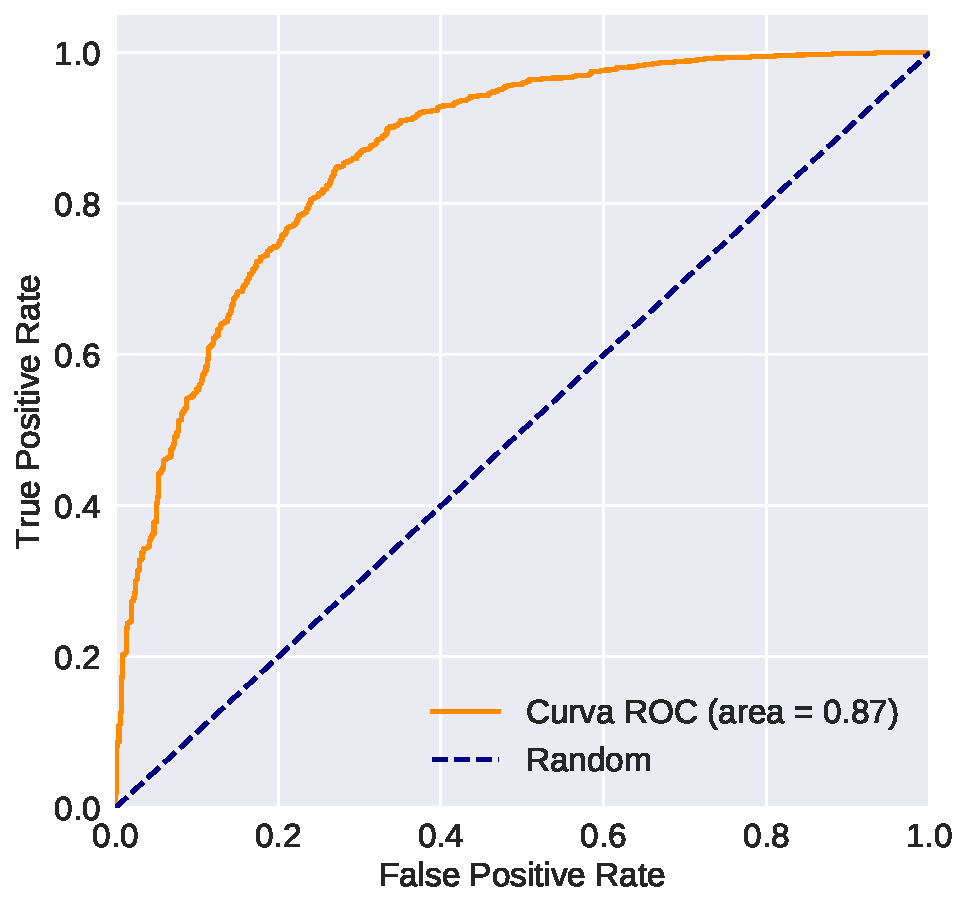
\includegraphics[width=\textwidth]{documents/latex/figures/3/integral_varq/auc_varq_integral.pdf}
    \caption{Curva AUC del algoritmo Random Forest y XGBoost del dataset Integral+VarQ Curado. La línea punteada corresponde a un predictor Random.}
    \label{fig:auc_integral_varq}
\end{subfigure}
\hfill
\hfill
\begin{subfigure}[b]{0.7\textwidth}
    \centering
    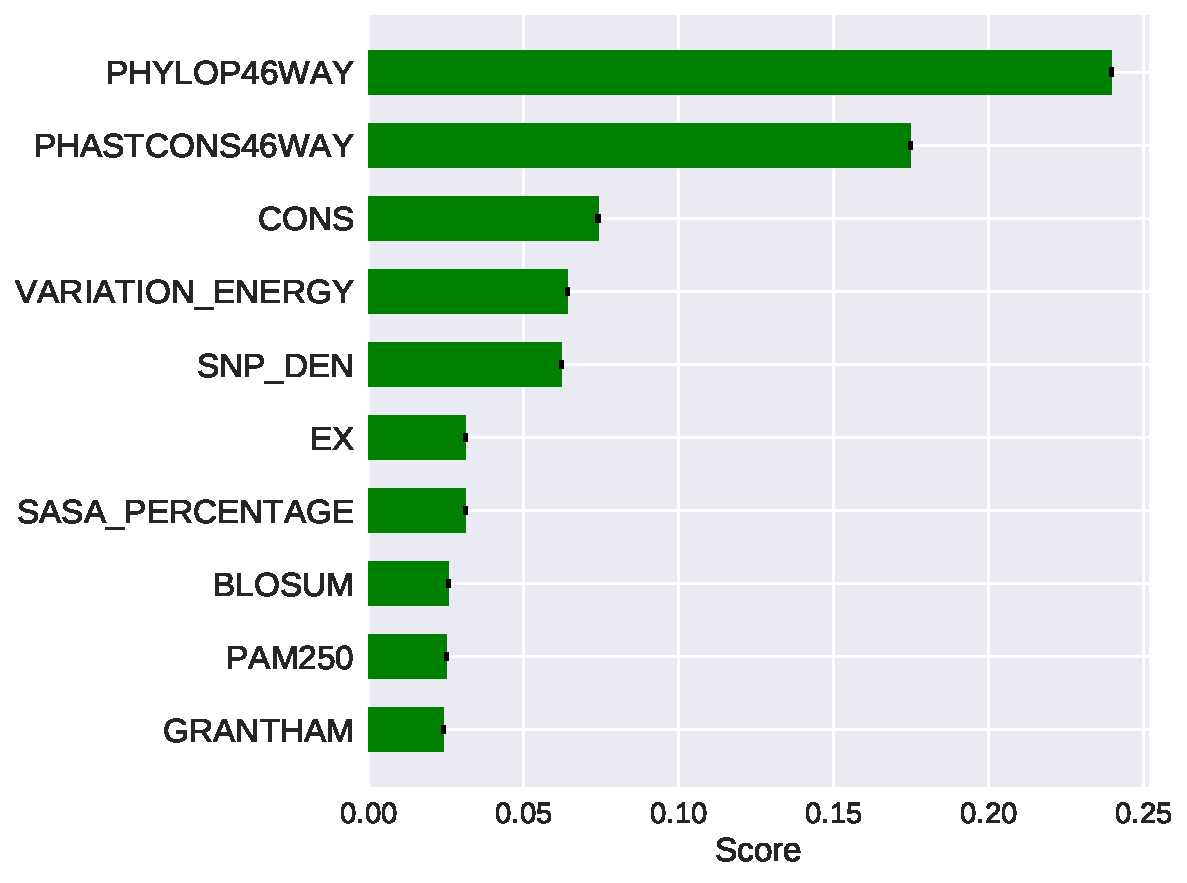
\includegraphics[width=\textwidth]{documents/latex/figures/3/integral_varq/importances_varq_integral.pdf}
    \caption{Los 10 atributos más importantes del dataset Integral+VarQ Curado usando Random Forest.}
    \label{fig:importances_integral_varq}
\end{subfigure}

\caption{Curva AUC y atributos más importantes del dataset Integral+VarQ Curado.}
\end{figure}
